\documentclass[Implementering/Implementering_main.tex]{subfiles}

\begin{document}

\section{Layout}
Dette afsnit præsenterer de eksterne værktøj, der er blevet anvendt på applikationens GUI.


\subsection{FontAwesome}
FontAwesome\footnote{https://fontawesome.com/cheatsheet} bliver brugt for de forskellige ikoner, som bliver brugt på applikationen, som kan ses på \ref{fig:FontAwesomeIcons}. 

\begin{figure}
    \centering
    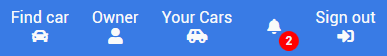
\includegraphics{Implementering/Graphic/FontAwesome.png}
    \caption{FontAwesome ikoner på navigationsbar, med tekst som har Roboto font}
    \label{fig:FontAwesomeIcons}
\end{figure}


\subsection{Roboto}
Roboto\footnote{https://fonts.google.com/specimen/Roboto} er den font, som bliver brugt til alt tekst i CarnGo Applikationen. I billag \textbf{Kravspecifikation} er der et ikke funktionelt krav, som siger at applikationen skal have en gratis font, og det er Roboto. 







\end{document}